\chapter{Использование и тестирование}

\section{Практическое применение программы}

Минимальная конфигурация для запуска приложения требует наличия виртуальной машины Java версии не ниже 1.7. Оптимальным выбором является Oracle HotSpot JVM.

Для учебных и исследовательских целей полезно работать напрямую с планировщиком, без стадии выполнения плана. Это требуется например, для проверки корректности его работы. Специальный класс \lstinline{PlanExport} позволяет построить план в виде описания графа на языке DOT и его изображения по заданному описанию на языке PDDL.

Доступ к классу осуществляется с помощью командной строки. Необходимо установить утилиту командной строки и сопутствующие библиотеки языка Scala. Следующая команда позволит сгенерировать условный план по описанию, содержащемуся в файле \texttt{bulb.pddl}. Результат работы будет помещен в файлы \texttt{plan.dot, plan.png}:

\begin{verbatim}
 scala com.glowingavenger.plan.importexport.PlanExport bulb.pddl plan.dot
\end{verbatim}

Доступен также примитивный диалоговый агент с пользовательским интерфейсом, построенным на основе диалоговых окон библиотеки Swing. При выполнении плана для каждого вопроса отображается окно вида:

\begin{figure}[h]
 \centering
 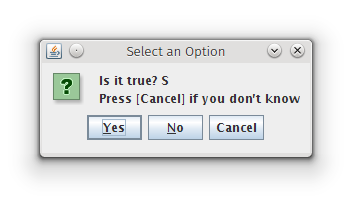
\includegraphics{snapshot1}
 \caption{Окно для выбора ответа на вопрос}
\end{figure}

При необходимости выполнить действие выводится соответствующее сообщение:

\begin{figure}[h]
 \centering
 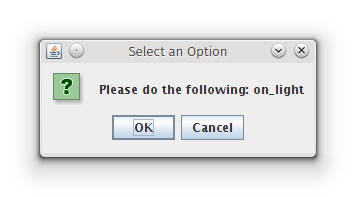
\includegraphics{snapshot2}
 \caption{Сообщение о необходимости выполнить действие}
\end{figure}

\section{Тестирование}

\subsection{Юнит-тесты}

\paragraph{FlatSpec + Matchers notation}

BDD\footnote{BDD - Behavior Driven Development}

\subsection{Нагрузочное тестирование}
\label{subsec:highload}

Для целей нагрузочного тестирование необходимо выполнить две задачи:

\begin{enumerate}
\item
  Сгенерировать случайным образом описание предметной области и проблемы
  на языке PDDL
\item
  Сделать замеры работы планировщика и определить узкие места алгоритмов
\end{enumerate}

\paragraph{Генерирование PDDL-описания}

В качестве параметров используются количество предикатов N, число
действий M, число аксиом L.

Введем правила наименования:

\begin{itemize}
\item
  Предикаты: P1, P2, \ldots{}
\item
  Действия: A1, A2, \ldots{}
\item
  Домены: D1, D2, \ldots{}
\item
  Проблемы: PR1, PR2, \ldots{}
\end{itemize}

Алгоритм создания случайного PDDL-описания рассмотрим на примере. Пусть
генерируется $K$-я предметная область, и $N=4, M = 2, L = 1$. Тогда
выполним следующие шаги:

\begin{enumerate*}
\item
  Запишем в результирующий файл описание предметной области и
  перечисление
  предикатов:
  \begin{verbatim}
   ( define (domain D1) (: predicates (P1) (P2) (P3) (P4) )
  \end{verbatim}

\item
  $M$ описаний действий. Под многоточием будем понимать логические
  формулы, алгоритм создания которых будет описан далее.
  \begin{verbatim}
   (: action A1 :precondition (...) :effect (...) )
   (: action A2 :precondition (...) :effect (...) )
  \end{verbatim}
  
\item
  $L$ описаний аксиом: \texttt{(: axiom (...) )}
\item
  Описание проблемы
  \begin{verbatim}   
   ( define (problem PR1)
    (: domain D1 )
    (: init (...) )
    (: goal(...) )
   )
  \end{verbatim}
\end{enumerate*}

Алгоритм генерирования логических выражений следующий:

\begin{enumerate*}
\item
  Выбрать (случайным образом) $n, 1 < n < N$.
\item
  Найти слуйчаное двоичное число из $N$ знаков с $n$ единицами $R_1$.
\item
  Найти случайное троичное число $(0, 1, 2)$ из $n$ знаков $R_2$.
\item
  Из множества всех предикатов $\{P_i\}$ выбрать те, для которых $i$-я
  позиция в $R_1$ равна единице. Обозначим их через $\{P_j\}$.
\item
  Заменить каждый из выбранных предикатов в соответствии с цифрой на
  $j$-й позиции в числе $R_2$. Так, $0$ соответствует $P_j$,
  $1 - \neg P_j$, $2 - P_j \vee \neg P_j$ или сокращенно, $P_j?$.
\item
  Взять конъюнкцию по всем полученным выражениям.
\end{enumerate*}

Пример для $N=4$:

\begin{enumerate*}
 \item $n=3$
 \item $R_1=1011$
 \item $R_2=102$
 \item $\{P_j\}=\{P_1, P_3, P_4\}$
 \item $P_1 \implies P_1, P_2 \implies \neg P_2, P_3 \implies P_3?$
 \item $P_1 \wedge \neg P_2 \wedge P_3?$
\end{enumerate*}


Генератор имеет программный интерфейс:

\begin{lstlisting}
    public interface PDDLGenerator {
        String[] generate(int predicates, int actions, int axioms);
    }
\end{lstlisting}

И может быть вызван из командной строки:

\begin{verbatim}
~# java com.glowingavenger.highload.PDDLGenerator out.pddl 10 10 3
\end{verbatim}

Здесь значения 10, 10, 3 находятся на тех же позициях, что и в методе
\texttt{generate}, а результат будет записан в файл \texttt{out.pddl}.

\paragraph{Измерение скорости работы}

Бенчмарк. Профайлер
